\documentclass[twoside]{article}
\setlength{\oddsidemargin}{0.25 in}
\setlength{\evensidemargin}{-0.25 in}
\setlength{\topmargin}{-0.6 in}
\setlength{\textwidth}{6.5 in}
\setlength{\textheight}{8.5 in}
\setlength{\headsep}{0.75 in}
\setlength{\parindent}{0 in}
\setlength{\parskip}{0.1 in}

\usepackage{graphicx}
\usepackage{url}

%
% The following commands sets up the lecnum (lecture number)
% counter and make various numbering schemes work relative
% to the lecture number.
%
\newcounter{lecnum}
\renewcommand{\thepage}{\thelecnum-\arabic{page}}
\renewcommand{\thesection}{\thelecnum.\arabic{section}}
\renewcommand{\theequation}{\thelecnum.\arabic{equation}}
\renewcommand{\thefigure}{\thelecnum.\arabic{figure}}
\renewcommand{\thetable}{\thelecnum.\arabic{table}}
\newcommand{\dnl}{\mbox{}\par}

%
% The following macro is used to generate the header.
%
\newcommand{\lecture}[4]{
  \pagestyle{myheadings}
  \thispagestyle{plain}
  \newpage
  \setcounter{lecnum}{#1}
  \setcounter{page}{1}
  \noindent
  \begin{center}
  \framebox{
     \vbox{\vspace{2mm}
   \hbox to 6.28in { {\bf CMPSCI~630~~~ Systems
                       \hfill Fall 2014} }
      \vspace{4mm}
      \hbox to 6.28in { {\Large \hfill Lecture #1  \hfill} }
%       \hbox to 6.28in { {\Large \hfill Lecture #1: #2  \hfill} }
      \vspace{2mm}
      \hbox to 6.28in { {\it Lecturer: #3 \hfill Scribes: #4} }
     \vspace{2mm}}
  }
  \end{center}
  \markboth{Lecture #1: #2}{Lecture #1: #2}
  \vspace*{4mm}
}

%
% Convention for citations is authors' initials followed by the year.
% For example, to cite a paper by Leighton and Maggs you would type
% \cite{LM89}, and to cite a paper by Strassen you would type \cite{S69}.
% (To avoid bibliography problems, for now we redefine the \cite command.)
%
\renewcommand{\cite}[1]{[#1]}

% \input{epsf}

%Use this command for a figure; it puts a figure in wherever you want it.
%usage: \fig{NUMBER}{FIGURE-SIZE}{CAPTION}{FILENAME}
\newcommand{\fig}[4]{
           \vspace{0.2 in}
           \setlength{\epsfxsize}{#2}
           \centerline{\epsfbox{#4}}
           \begin{center}
           Figure \thelecnum.#1:~#3
           \end{center}
   }

% Use these for theorems, lemmas, proofs, etc.
\newtheorem{theorem}{Theorem}[lecnum]
\newtheorem{lemma}[theorem]{Lemma}
\newtheorem{proposition}[theorem]{Proposition}
\newtheorem{claim}[theorem]{Claim}
\newtheorem{corollary}[theorem]{Corollary}
\newtheorem{definition}[theorem]{Definition}
\newenvironment{proof}{{\bf Proof:}}{\hfill\rule{2mm}{2mm}}

% Some useful equation alignment commands, borrowed from TeX
\makeatletter
\def\eqalign#1{\,\vcenter{\openup\jot\m@th
 \ialign{\strut\hfil$\displaystyle{##}$&$\displaystyle{{}##}$\hfil
     \crcr#1\crcr}}\,}
\def\eqalignno#1{\displ@y \tabskip\@centering
 \halign to\displaywidth{\hfil$\displaystyle{##}$\tabskip\z@skip
   &$\displaystyle{{}##}$\hfil\tabskip\@centering
   &\llap{$##$}\tabskip\z@skip\crcr
   #1\crcr}}
\def\leqalignno#1{\displ@y \tabskip\@centering
 \halign to\displaywidth{\hfil$\displaystyle{##}$\tabskip\z@skip
   &$\displaystyle{{}##}$\hfil\tabskip\@centering
   &\kern-\displaywidth\rlap{$##$}\tabskip\displaywidth\crcr
   #1\crcr}}
\makeatother

% **** IF YOU WANT TO DEFINE ADDITIONAL MACROS FOR YOURSELF, PUT THEM HERE:



% Some general latex examples and examples making use of the
% macros follow.

\begin{document}

%FILL IN THE RIGHT INFO.
%\lecture{**LECTURE-NUMBER**}{**DATE**}{**LECTURER**}{**SCRIBE**}
\lecture{3}{September 9}{Emery Berger}{Shaylyn Adams, Nick Braga}

\section{Runtime Systems}

%Insert figure HERE

\underline{Runtime system} is generic term that refers to the ''grab bag'' of support features for the programming language. Examples include:
\begin{itemize}
\item[-] Garbage collection
\item[-] Memory management (malloc, free, realloc, etc.)
\item[-] Libraries (C library, libc.so, libstdc++.so, etc.)
\item[-] Threads
\end{itemize}

\section{Garbage Collection}
The paper examined for today's class, ''Garbage collection in an uncooperative environment'' (Boehm et al., 1991), set out to make a stand-alone/external garbage collector that did not need to cooperate with the compiler/interpreter.

Garbage collectors can be broken down into two different categories; \textbf{precise} and  \textbf{conservative}.
\begin{description}
\item[Precise] This indicates a GC environment where all pointers are \underline{known}. Real pointers \(\cap \) discovered pointers = real pointers.
\begin{verbatim}
class foo{
		int x; ------->NOT a pointer 
		int y; ------->NOT a pointer 
		char s; ------->NOT a pointer 
		String st; ------->YES a pointer to another object! (keeps track of this one)
	}
\end{verbatim}
Writing efficient, concurrent GC is difficult to do with stack maps which is where conservative GC comes in. 
\item[Conservative] As expected, this does not keep track of pointers in the same way as precise GC. Here, we have to determine if something is a pointer. It is considered to be 'conservative' because memory will never be reclaimed too soon. \pagebreak
\begin{center}
\centering
\begin{tabular}{cccccccc}
\hline
\textbar & \textbar & \textbar  & \textbar & \textbar & \textbar & \textbar & \textbar \\
\hline
\end{tabular} \\
min \hspace{72pt} max
\end{center}
To discover the pointers, conservative GC will look through the allocated memory block, which has a minimum and maximum address range. If the object is not found within this range, then it cannot be a pointer. If it is within the range, a second check must occur as an attempt to catch any integers that look like an address. This check is for alignment, since every pointer \underline{has} to be a multiple of 4 or 8, i.e. \%4=0 or \%8=0 (otherwise it is not a pointer). Thus, if the address is in range and it is also correctly aligned, the GC must treat it as a pointer. \\

However, it is still possible for a supposed pointer to actually be an integer that is in the range and divisible by 4 or 8. Generally, if a chain of pointers is followed and goes off into nowhere, it is safe to assume that it is not a pointer and it can be put on the  \underline{blacklist} in which no memory will ever be allocated from again. (JavaScript on Internet Explorer uses conservative garbage collection to this day.)
\end{description}
\subsection{Mark-Sweep Garbage Collection}
Mark-sweep garbage collection is the GC algorithm that recursively marks all reachable nodes black, and sweeps for white (unblackened) nodes that will be reclaimed (since anything unreachable needs to be reclaimed). After, it will color reachable nodes 'white' and go through the process again. Variables that indicate color correspondence are maintained. \\

\emph{Aside}: The BiBop(= big bag of pointers) allocator achieves a lazy sweep process by keeping things in many big chunks with a bit map to indicate what is in use/allocated.
	
\subsection{Stop the World Garbage Collection}
The 'original' type of garbage collection is known as \textbf{Stop-the-world}, where the program would sit and stop, or \emph{pause}, while garbage collection was performed. This pause will obviously take longer depending on the size of the heap. It is a linear process and there is no way around it. Hence, garbage collection received a bad reputation as being incredibly slow. There are other forms of garbage collection such as concurrent, parallel, and incremental, but regardless the garbage collector has to check all nodes/pointers or use a heuristic that keeps track of pointer sections. The type of garbage collector to strive for is one that is fast and happens rarely.

\subsection{Garbage Collection Properties}
There are 2 properties to be aware of when constructing a garbage collector and it is important to reach a balance between the two of them.
\begin{description}
\item{1) Soundness} = no reachable memory is ever reclaimed. If you never ran a garbage collector you would achieve ultimate soundness.
\item{2) Completeness} = all unreachable is eventually reclaimed.
\end{description}


\subsection{Problems with Garbage Collection}
The biggest problem with conservative garbage collection and using mark-sweep is that it can result in a porous (fragmented) memory space, requiring:
\begin{enumerate}
\item[1)]More space (which in turn impacts the cache)
\item[2)] Underlying architecture optimizations
\end{enumerate}

\begin{description}
\item[Locality] the property that defines objects' proximity to one another in the memory space. 
\end{description}
There are two types of locality:
\begin{itemize}
\item[1)] Spacial locality: Similar items should be stored in the closest proximity feasible. For example, if we use byte 1, it is likely that we'll also use byte 2 in practice)
\item[2)] Temporal locality: items should be used in a close time range, before objects are then changed again
\end{itemize}
The GC cannot choose specific objects to keep in RAM, and therefore must sends 'chunks' of data to the cache. Fetching memory is expensive and can incur a penalty of around 100 cycles.\\
One technique to this end could be to move pointers (compaction). The problem with compaction is that it is possible to overwrite integers by doing so. Since there is no cooperation with the programming language, conservative garbage collection cannot move objects easily. Conservative GC will only reclaim pointers, but might accidentally overwrite in this way. It can find integers that look that addresses and then would end up trashing real memory.

\emph{Aside}: \begin{quotation}"All problems in computer science can be solved by another level of indirection" -\begin{small}David Wheeler\end{small}\\
Corollary: "...except for the problem of too many layers of indirection." -\begin{small}Kevlin Henney\end{small}
\end{quotation}

This problem of moving pointers can be solved with \textbf{handles}. Handles make it easier to reallocate memory; this is because only the 'handle table' points to actual objects. It is theoretically a pretty good solution but can be expensive.  The number of operations is multiplied whenever an object is dereferenced, resulting in poor performance in practice. If you can allocate relatively small amounts of memory, GC overhead can be made small. This is not possible with handles. Handles tend to interact poorly with \textbf{prefetchers} since handles are unpredictable and the next move cannot be predicted at the architecture level even with smart prefectchers. (One example of a prefetcher is a \underline{stride prefetcher}, which learns loops by observing the memory stream).

In conclusion, while conservative GC cannot overcome fragmentation, using handles has other performance overheads above conservative GC.
\subsection{Garbage Collection Evolution Timeline}
Everyone is always trying to 'reinvent the wheel'.
\begin{center}
\textsc{Interpreter}: {\scriptsize Perl, PHP, Ruby, Python, JavaScript, etc., all easy to write}-------\textgreater \textsc{terrible GC}: {\scriptsize reference counting}-------\textgreater \textsc{mark-sweep}: {\scriptsize better GC}-------\textgreater \textsc{Just in time Compiler}: {\scriptsize Interpreter is too slow}-------\textgreater \textsc{"Fancy GC"}: {\scriptsize Typically doesn't work}
\end{center}
\begin{scriptsize}
a): In this diagram, each memory-allocated unit contains both a data bucket and a reference counting bucket. The garbage collector has determined an unreachable node (marked in red) and has reclaimed the memory space, also removing its pointer(s) and decrementing its reference count. (b): The GC then recursively moves through the reclaimed node's pointer from (a), and reclaims if unreachable, etc.)\\
\end{scriptsize}


\textbf{Reference} \textbf{counting} is a type of GC where all incoming pointers are kept track of. So, on every single pointer update the RC destination must be increased and the RC origin must be decreased. If RC count==0, recursively decrement references of all things after and then reclaim object. However, with circular objects like doubly linked lists, reference counting will not work.(Object(ionable)ive C uses explicit reference counting where the programmer must do it manually.)
\begin{figure}
\centering
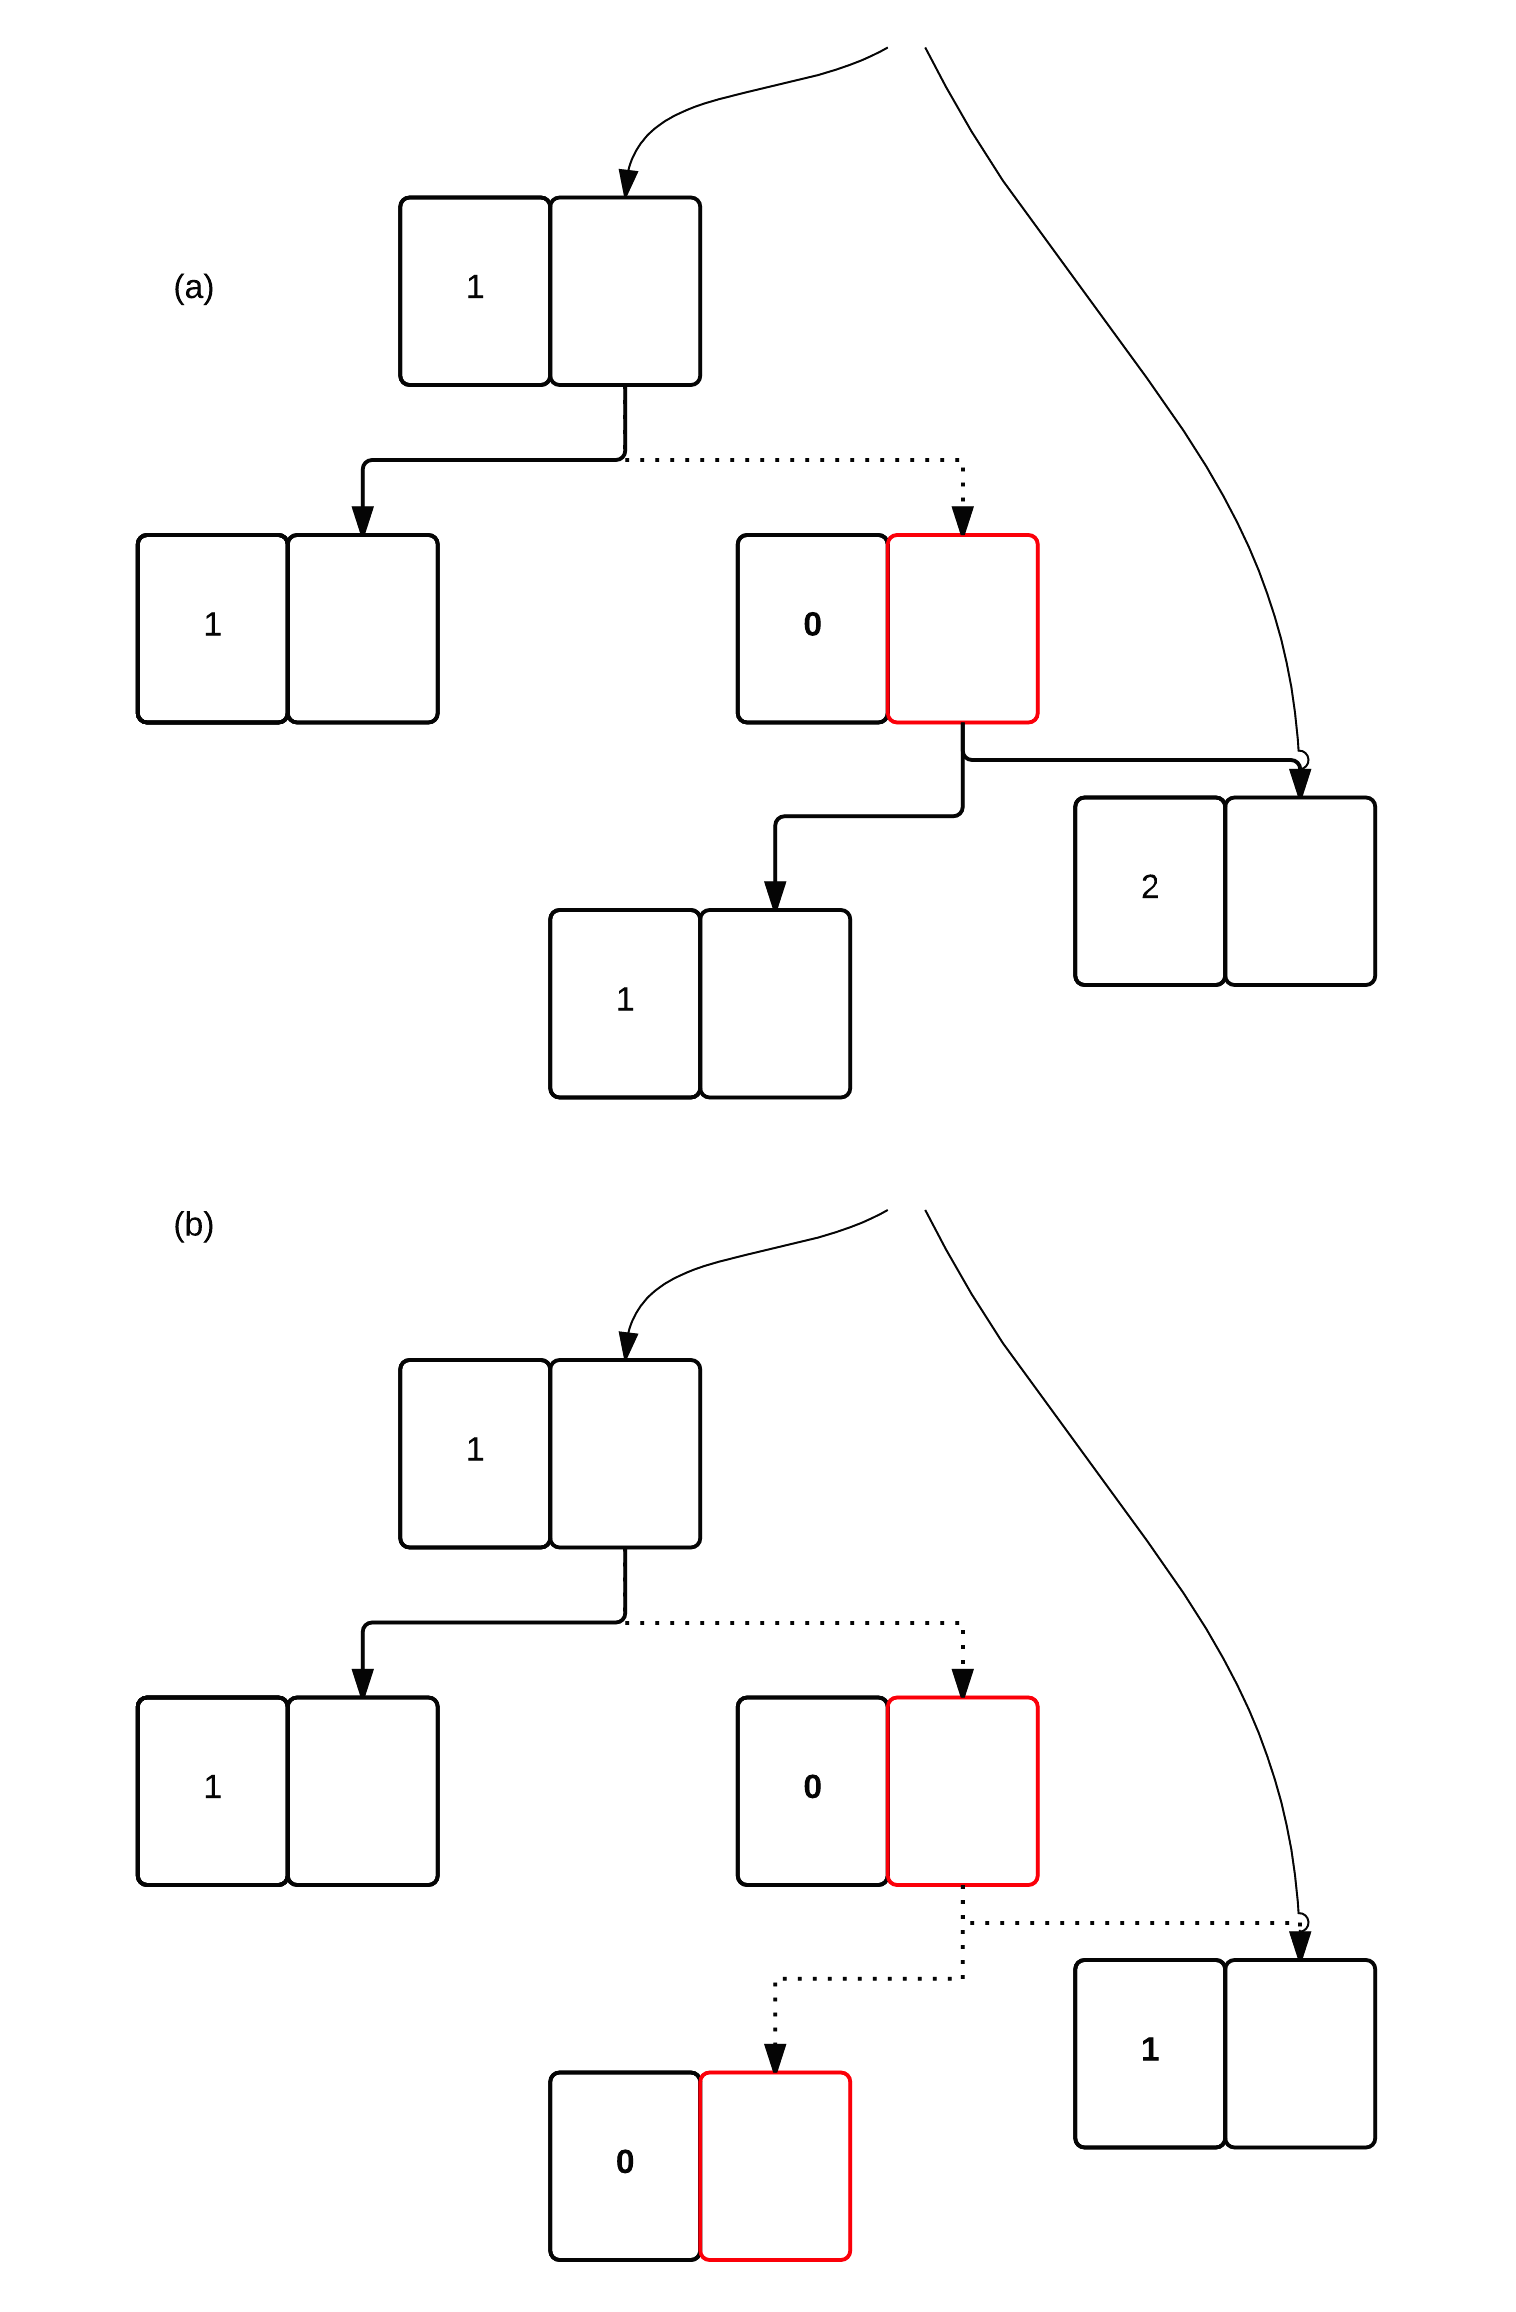
\includegraphics[width=70mm]{Original.png}
\end{figure}

\emph{Aside}:  \underline{Vaporware} refers to software that is announced but never materializes.
\subsection{Running out of Memory and Swapping Tangent}

\underline{OOM-Killer}, or out of memory killer, refers to the Linux nuance where when memory capacity is reached, the kernel will pick an unsuspecting victim to "kill" based on a heuristic. Ironically, Linux used to always effectively commit suicide by killing process 0 aka the kernel itself.\\
-Disk \underline{swapping }via LRU frees up physical memory. \\
-\underline{Paging/thrashing} refers to the process of constantly moving memory back and forth from disk when RAM is full. \\
-There is no  swap space in iOS.\\
-Linux used to overcommit memory even when there was not enough swap room.

\end{document}
